\chapter{Исследовательская часть}

\section{Технические характеристики}

Технические характеристики устройства, на котором выполнялись замеры по времени:

\begin{itemize}
    \item Процессор: Intel i5-1035G1 (8) @ 3.600GHz.
    \item Оперативная память: 16 ГБайт.
    \item Операционная система: Manjaro Linux x86\_64 (версия ядра Linux 5.15.131-1-MANJARO).
\end{itemize}

Во время проведения измерений времени ноутбук был подключен к сети электропитания и был нагружен только системными приложениями.

\section{Демонстрация работы программы}

На рисунке \ref{fig:prog-demo} показан пример работы разработанной программы для случая, когда пользователь выбирает действие <<Запуск алгоритмов поиска расстояния Левенштейна>> и вводит строки <<кот>> и <<кошка>>.

\clearpage
\begin{figure}[h]
    \centering
    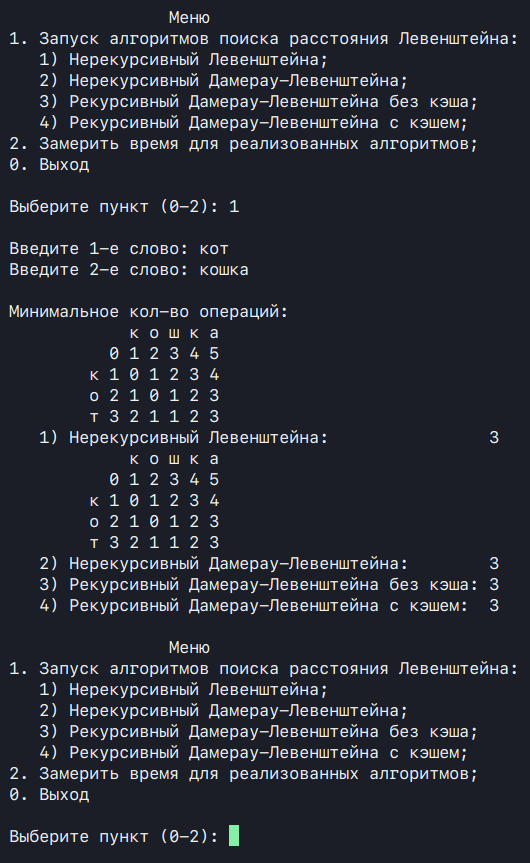
\includegraphics[height=0.7\textheight]{images/prog_demo.png}
    \caption{Демонстрация работы программы}
    \label{fig:prog-demo}
\end{figure}

\section{Временные характеристики}

Исследование временных характеристик алгоритмов производилось на случайно сгенерированных строках длинами от 1 до 10, длины изменяются с шагом 1. Для нерекурсивных алгоритмов отдельно производилось сравнения на строках длинами от 20 до 100 с шагом изменения длины 10. Во избежание погрешности измерения для каждой строки производились 50 раз, затем вычислялось среднее арифметическое всех полученных значений времени.

\section{Характеристики по памяти}

\section{Вывод}